\section{Beschleuniger-Massensepektrometrie}

Massensektrometrie ist ein Verfahren mit dem die Masse ($m/q$) von Atomen oder Molekülen aus einer Probe gemessen werden kann.
Bei Beschleuniger-Massenspektrometrie wird dies von einem Teilchenbeschleuniger unterstützt, indem die Teilchen aus der Probe auf hohe Energien beschleunigt werden.
Ein Vorteil dieser Methode ist es, dass Kernisobare (z. B. $^{10}$Be und $^{10}$B) separiert werden können und dass auch geringe Mengen eines Isotops nachgewiesen werden können.
Im Folgenden wird eine detaillierte Beschreibung des Vorgehens anhand des DREAMS (DREsden Accelerator Mass Spectrometer) am HZDR gegeben.

\begin{figure}[ht]
  \includegraphics[width=\linewidth]{../Bilder/dreams.png}
  \caption{Darstellung des Beschleuniger-Massenspektrometrie-Aufbaus am HZDR [Quelle]}
  \label{dreams}
\end{figure}
Wir betrachten als Beispiel die Messung des Isotopenverhältnisses von  $^{10}$B und  $^{10}$Be.
Die chemisch aufbereitete Probe befindet sich am Anfang in einer Sputter-Ionenquelle.
Cäsiumatome werden erhitzt, dabei ionisiert und mithilfe einer angelegten Spannung von 7 kV auf die Probe beschleunigt.
Dabei werden Atome aus dieser gelöst und nehmen Elektronen auf.
Durch eine angelegte Spannung von 29 kV werden die entstandenen negativen Ionen jetzt beschleunigt.
Mithilfe eines elektrischen Feldes am ESA (elektrostatischer Deflektor) und eines magnetischen Feldes am $90^{\circ}$ Magneten werden dabei Ionen unerwünschter Masse herausgefiltert.
An dieser Stelle wird z. B. das Isotop  $^{9}$B aus dem Strahl entfernt.
Im Strahl verbleiben das Radioisotop $^{10}$Be und das stabile Isotop $^{10}$B
Dieser negative Ionenstrahl, wird danach mit einer Spannung von bis zu $6$ MV in die Mitte des Tandem beschleunigt, in welchem sich ein Argon-Gas befindet.
Durch Wechselwirkungen der Ionen mit dem Gas und durch die herrschenden Energien werden verbleibende Moleküle zerstört und Elektronen aus den Ionen geschlagen.
Die jetzt positiven Ionen werden im Tandem weiter zur anderen Seite beschleunigt.
Die Energie der Teilchen nach dem Tandem kann berechnet werden mit:
\begin{equation}
E = e \cdot (U_{IonSource + U_{Acc}} \cdot \frac{m_{ion^+}}{m_{mol^-}} + U_{Acc}\cdot q_{ion})
\end{equation}
Mit der Elementarladung $e$, der Spannung an der Ionenquelle $U_{IonSource}$, der Spannung am Tandem $U_{Acc}$, der Ionenmasse $m_{ion^+}$, der Masse der Moleküle $m_{mol^-}$ und dem Ladungszustand der Ionen $q_{ion}$.
Dort wartet ein weiterer $90^{\circ}$ Magnet, durch dessen magnetisches Feld die Isotope nach Masse getrennt werden.
Stabile Isotope ($^{10}$B) können jetzt mithilfe eines Faraday-Cup gemessen werden.

Für die Messung der radioisotope ergibt sich jetzt das Problem, dass einzelne $^{10}$B Isotope aufgrund im Strahl verbleiben, was die weitere Messung stören würde..
Um diese Isobare rauszufiltern wird eine dünne Siliciumnitrid-Folie in den Weg des Strahls gelegt.
Der Energieverlust von schweren geladenen Teilchen in dieser Folie berechnet sich mit:
\begin{equation}
E_{loss} = d \cdot \left( \frac{\Delta E}{\Delta x} \right)
\end{equation}
Mit der Dicke der Folie $d$ und dem teilchenspezifischen Energieverlust $\frac{\Delta E}{\Delta x}$.
Durch den massen- und ladungsabhängige Energieverlust der Teilchen in dieser, können dann die $^{10}$B Ionen, welche mehr Energie verlieren werden, mithilfe eines elektrischen Feldes in einem weiteren ESA aus dem Strahl entfernt werden
Gleichzeitig werden innerhalb der Folie weitere Elektronen herausgeschlagen, wodurch die Ladung weiter positiv wird (z. B. $^{10}B^{4+}$).
Ein weiterer Magnet lenken den Strahl dann zu einer Gasionisationskammer (AMS gas-filled ionization chamber in Ab. \ref{dreams}), indem die Ionen mithilfe von vier Anoden (A, B, C, D) in einem Isobutengas ($C_{4}H_{10}$) gezählt werden (siehe Abb. \ref{ion_chamber}).
\begin{figure}[ht]
  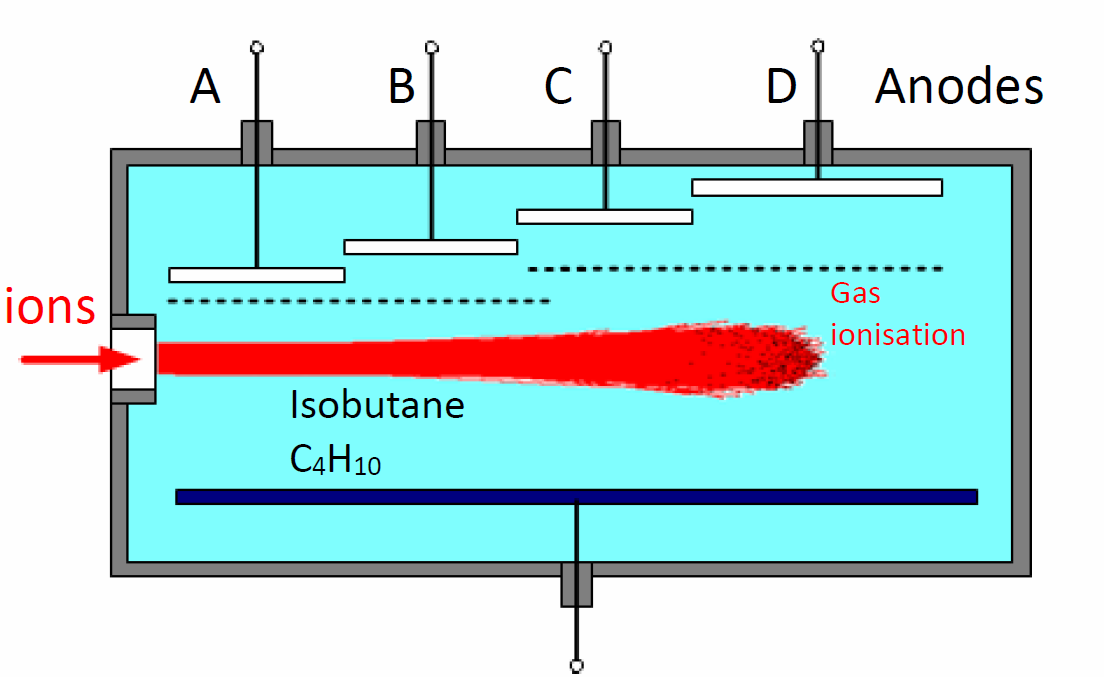
\includegraphics[width=\linewidth]{../Bilder/ion_chamber.png}
  \caption{Gasionisationskammer am DREAMS [Quelle]}
  \label{ion_chamber}
\end{figure}
\clearpage
